\chapter{Service Work}
\label{sec:service_work}
\section{\susyv2 Analysis Framework}
\susyv2 is a standalone, \root-based analysis framework. Analysis
scripts are written in the Python programming language. These make use of
low-level, high-performance classes written in C++. This provides a good
compromise between speed and flexibility.

The \susyv2 package has been used for a number of analyses at
\ac{CMS}. These have primarily been \ac{SUSY}-based analyses. It has also been
used for the \PW polarisation measurement as well as several other projects. The
vast majority of the initial code was written by Dr. John Jones with subsequent
contributions from a number of others.

The \susyv2 code aims to minimise the number of reads performed on a \root tree
by reading branches on demand and performing lazy calculations as required to
satisfy analysis code requests for higher-level observables. The dependency
chain between calculated quantities may be viewed as a tree. The leaves of this
tree correspond to quantities stored directly in the \root file (or an
alternative serialisation format). To minimise computation, each node in this
tree performs its calculation (or \ac{IO} in the case of the leaf nodes) only
once per event. The results are then cached. Subsequent use of this quantity
then returns the cached result directly. Furthermore, access to quantities
dependent on others which have already been calculated will require the minimum
necessary calculation, reutilising cached values and minimising further \ac{IO}
or CPU usage.

As well as the performance advantages of this approach, it has the benefit of
enforcing a kind of ``referential transparency'' -- repeated access to a given
quantity must always yield the same result (at the single-event level). Whilst
this makes certain tasks more involved -- e.g. iterative cleaning of events --
it ensures that analysis selections must ``commute'' - since they are unable to
mutate any of the quantities on which they select. This emulates some of the
benefits available in purely functional programming languages such as
Haskell~\cite{history_of_haskell}.

My contributions were in the maintenance and development of this code-base, the
addition of a flexible Python-based configuration system, support for the \root
\textsc{TChain} class, infrastructure for managing and monitoring batch
submissions, and the implementation of a fast ``cross-cleaner''. The
cross-cleaner must resolve ambiguties between physics objects. The detected
ambiguities may form cyclic graphs, which require careful resolution.

\section{The \acl{GCT}}
\label{sec:l1t}
The \ac{GCT}, previously been described in \sec~\ref{sec:l1t}, formed the focus
of my service work during the PhD. This followed on from previous work on the
``jet-finder'' component which formed the basis of my MSci project.

As well as undertaking shift-work and on-call duties I was responsible for
debugging problems experienced before the start of data-taking with the
\emph{source card} components. These boards receive data from the \ac{RCT} and
then transmit it, via optical fibres, to the \emph{leaf cards} of the
\ac{GCT}. The data is organised in a manner suited to the processing performed
by the \ac{GCT}. The data is received from the \ac{RCT} on $6\times 68$ pin
differential \ac{ECL} \ac{SCSI} cables running at \unit{80}{\mega\hertz}. Errors
were occurring intermittently in pattern tests run at the experimental service
cavern. These problems could not be reproduced in the test setup. It was
eventually discovered that the errors were caused by deficiencies in the
\ac{SCSI} cables linking the source cards to the \ac{RCT}. The problematic
cables were replaced, eliminating the errors.

I was also responsible for testing a hardware implementation of an improved
\ac{L1T} tau algorithm. This is illustrated in \fig~\ref{fig:l1t_tau_algo}. In
addition to, or instead of the use of the tau veto bit (see \sec~\ref{sec:l1t}),
an isolation requirement is placed on the tau-jet. To be classified as a tau,
seven of the eight surrounding regions must be below a programmable
threshold. This is found to reduce the rate by a factor of two, whilst
maintaining efficiency. The algorithm was added to the firmware present on the
\acp{FPGA} in the \ac{GCT}'s leaf cards. I was responsible for testing the
algorithm in hardware. Firstly, a test suite written in the Python programming
language was used to generate many combinations of energy patterns. These were
then run through the hardware in order to verify that the basic implementation
was correct. It was then subsequently tested with a number of random patterns. A
software emulation of the hardware was used to verify the results. A number of
problems were found both in the hardware implementation and in the consistency
of the emulator and hardware. These problems were subsequently fixed.

\begin{figure}
\centering
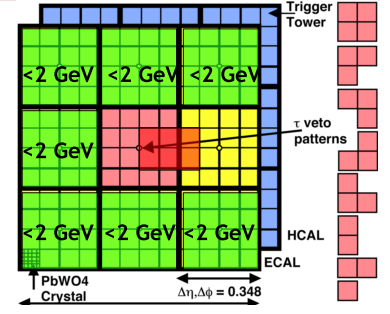
\includegraphics[width=0.5\textwidth]{fig/new_tau_algo}
\caption[]{Illustration of the improved tau algorithm at the \ac{L1T}. A
  $3\times 3$ region sliding window algorithm is used to find jets. Tau-jets are
  identified as those for which none of the nine tau-veto bits are set. The
  improved algorithm augments or replaces this requirement with an isolation
  cut. Seven of the eight regions surrounding the central location must be below
  a programmable threshold -- here set to \unit{2}{\GeV}.}
\label{fig:l1t_tau_algo}
\end{figure}
